\chapter{METHODOLOGY}
\label{ch:methodology}

This chapter details the proposed Learnable Polynomial Approximation Network (LPAN) framework for achieving secure Transformer inference using Fully Homomorphic Encryption (FHE). We first describe the system architecture and polynomial approximation foundations, then present each methodological contribution in detail.

\section{System Architecture}
The privacy-preserving framework operates on a client-server model. The client encrypts the initial prompt using a public key before transmitting it to the cloud server. The server, hosting the LLM weights in plaintext, processes the encrypted embeddings using homomorphic addition and multiplication operations. The resulting encrypted output tokens are returned to the client, who decrypts them using the corresponding secret key.

Figure~\ref{fig:client_server} illustrates the encrypted inference protocol between the client and the cloud server.

\begin{figure}[htbp]
\centering
\begin{tikzpicture}[
    box/.style={draw, rounded corners=3pt, thick, minimum width=2.8cm, minimum height=1cm, align=center, font=\small},
    clientbox/.style={box, fill=green!15, draw=green!50!black},
    serverbox/.style={box, fill=blue!12, draw=blue!50!black},
    databox/.style={draw, rounded corners=2pt, thick, minimum width=2.2cm, minimum height=0.6cm, font=\scriptsize, align=center},
    arr/.style={-{Stealth[length=3mm]}, very thick},
    note/.style={font=\scriptsize, text=gray!70!black},
]

% Client side
\node[clientbox, minimum width=3.5cm, minimum height=1.2cm] (client) at (0, 0) {\textbf{Client}};
\node[note, anchor=west] at (2.0, 0) {Holds secret key $sk$};

% Server side
\node[serverbox, minimum width=3.5cm, minimum height=1.2cm] (server) at (10, 0) {\textbf{Cloud Server}};
\node[note, anchor=east] at (8.0, 0) {Holds model weights $W$};

% Step 1: Key generation
\node[databox, fill=green!10] (keygen) at (0, 3.0) {Key Generation};
\node[note, anchor=west] at (1.5, 2.3) {$(pk, sk, evk) \leftarrow \mathrm{KeyGen}()$};

% Step 2: Encrypt
\node[databox, fill=green!10] (encrypt) at (0, -2.5) {Encrypt Input};
\node[note, anchor=west] at (1.5, -3.2) {$\mathit{ct}_x = \mathrm{Enc}(pk, \mathbf{x})$};

% Step 3: Send encrypted data + eval key
\draw[arr, green!60!black] (2.0, -2.2) -- node[above, font=\scriptsize, sloped] {$\mathit{ct}_x$, $pk$, $evk$} (8.0, -2.2);

% Step 4: Homomorphic computation
\node[serverbox, minimum width=3.8cm, minimum height=2.6cm] (hcomp) at (10, -5.0) {};
\node[font=\small, text=blue!60!black] at (10, -4.1) {\textbf{HE Inference}};
\node[note, text width=3.2cm, align=center] at (10, -5.4) {
$\mathit{ct}_{h_1} = W_1 \cdot \mathit{ct}_x + b_1$\\
$\mathit{ct}_{h_2} = p_{\text{GELU}}(\mathit{ct}_{h_1})$\\
$\vdots$\\
$\mathit{ct}_y = f(\mathit{ct}_x; W)$
};

% Arrow from server to HE computation
\draw[arr, blue!50!black] (server.south) -- (hcomp.north);

% Step 5: Return encrypted result
\draw[arr, blue!50!black] (8.0, -7.2) -- node[below, font=\scriptsize, sloped] {$\mathit{ct}_y$ (encrypted prediction)} (2.0, -7.2);

% Step 6: Decrypt
\node[databox, fill=green!10] (decrypt) at (0, -7.2) {Decrypt};
\node[note, anchor=west] at (1.5, -7.9) {$\hat{y} = \mathrm{Dec}(sk, \mathit{ct}_y)$};

% Security boundary
\draw[dashed, thick, red!50] (5.0, 4.0) -- (5.0, -8.8);
\node[font=\scriptsize, text=red!60, rotate=90] at (5.5, -5.5) {Encryption Boundary};

% Trust zones
\node[font=\scriptsize\bfseries, text=green!50!black] at (0, 3.8) {TRUSTED};
\node[font=\scriptsize\bfseries, text=blue!50!black] at (10, 3.8) {UNTRUSTED};

% Arrows from client
\draw[arr, green!60!black, dashed] ([xshift=-0.5cm]client.north) -- ([xshift=-0.5cm]keygen.south);
\draw[arr, green!60!black, dashed] ([xshift=-0.5cm]client.south) -- ([xshift=-0.5cm]encrypt.north);
\end{tikzpicture}
\caption{Client-server protocol for privacy-preserving inference. The client encrypts the input using CKKS, sends the ciphertext and evaluation keys to the server. The server performs all Transformer computations homomorphically on encrypted data---never accessing plaintext. The encrypted result is returned to the client for decryption.}
\label{fig:client_server}
\end{figure}

Unlike prior frameworks (THE-X~\cite{chen2022thex}, MPCFormer~\cite{li2023mpcformer}, BOLT~\cite{pang2024bolt}) that require interactive communication during inference for non-linear operations, our framework produces a \emph{fully-polynomial} model where all operations---including LayerNorm---can be evaluated non-interactively within the CKKS scheme.


\section{Polynomial Approximation Foundations}
\label{sec:poly_approx}

As established in Section~\ref{sec:nonlinearity_bottleneck}, FHE schemes natively support only addition and multiplication. Every non-polynomial function in the Transformer must be replaced by a polynomial of bounded degree. This section develops the mathematical foundations of the three principal approximation strategies.

\subsection{Taylor Series Approximation}

The Taylor series expansion of a function $f(x)$ around a point $a$ provides a natural polynomial approximation:
\begin{equation}
    f(x) = \sum_{k=0}^{\infty} \frac{f^{(k)}(a)}{k!}(x - a)^k,
    \label{eq:taylor_general}
\end{equation}
with the truncation error bounded by:
\begin{equation}
    \left| f(x) - T_n(x) \right| \leq \frac{M_{n+1}}{(n+1)!} |x - a|^{n+1},
    \label{eq:taylor_error}
\end{equation}
where $M_{n+1} = \max_{\xi \in [a, x]} |f^{(n+1)}(\xi)|$. Taylor approximation converges rapidly near $a$ but diverges at interval boundaries---problematic for FHE where inputs are not tightly controlled after several encrypted layers.

\subsection{Minimax (Chebyshev) Approximation}

Minimax approximation seeks the polynomial of degree~$n$ that minimizes the maximum absolute error over an entire interval $[a, b]$:
\begin{equation}
    p_n^* = \arg\min_{p \in \mathcal{P}_n} \max_{x \in [a, b]} |f(x) - p(x)|.
    \label{eq:minimax}
\end{equation}
The Chebyshev Equioscillation Theorem guarantees that $p_n^*$ is unique and characterised by at least $n+2$ equioscillation points where the error alternates in sign.

Minimax approximations are computed in the Chebyshev polynomial basis $\{T_k(x)\}_{k \geq 0}$, defined by the recurrence:
\begin{align}
    T_0(x) &= 1, \quad T_1(x) = x, \label{eq:cheb_base} \\
    T_{k+1}(x) &= 2x \cdot T_k(x) - T_{k-1}(x), \quad k \geq 1. \label{eq:cheb_recurrence}
\end{align}
For an arbitrary interval $[a, b]$, the affine map $\hat{x} = \frac{2x - (a+b)}{b - a}$ transforms to $[-1, 1]$. Chebyshev coefficients are evaluated at runtime using the numerically stable Clenshaw recurrence:
\begin{equation}
    f(x) \approx \sum_{k=0}^{n} c_k\, T_k(\hat{x}), \quad \text{evaluated via } b_k = c_k + 2\hat{x}\, b_{k+1} - b_{k+2}.
    \label{eq:clenshaw}
\end{equation}

\subsection{Least-Squares Regression Approximation}

Least-squares regression minimizes the mean squared error:
\begin{equation}
    p_n^{\text{LS}} = \arg\min_{p \in \mathcal{P}_n} \int_{a}^{b} \left[f(x) - p(x)\right]^2 w(x)\, dx.
    \label{eq:least_squares}
\end{equation}
When the weight function $w(x)$ matches the empirical activation distribution, least-squares can outperform minimax in average error, though at the cost of potentially larger worst-case error at boundaries.

\subsection{Approximation of the Inverse Square Root for LayerNorm}

LayerNorm requires computing $1/\sqrt{\sigma^2 + \epsilon}$. Two HE-compatible strategies exist:

\paragraph{Direct polynomial approximation.} Fit a low-degree polynomial to $g(x) = 1/\sqrt{x}$ over the expected variance range $[\epsilon, V_{\max}]$:
\begin{equation}
    \widetilde{g}(x) = \alpha_0 + \alpha_1 x + \alpha_2 x^2 + \cdots + \alpha_n x^n.
    \label{eq:invsqrt_poly}
\end{equation}

\paragraph{Goldschmidt iteration.} Iteratively refine an initial estimate $y_0 \approx 1/\sqrt{x}$:
\begin{align}
    h_i &= 1 - x \cdot y_i^2, \label{eq:goldschmidt_h} \\
    y_{i+1} &= y_i \cdot \left(1 + \frac{h_i}{2}\right). \label{eq:goldschmidt_y}
\end{align}
Each iteration consumes 3--4 multiplicative levels. Our LPAN framework uses the direct polynomial approach with learnable coefficients, avoiding the depth cost of iterative methods.

\subsection{Multiplicative Depth Analysis}
\label{sec:depth_analysis}

A degree-$n$ polynomial can be evaluated in $\lceil \log_2 n \rceil$ multiplicative depths using a balanced evaluation tree. For the complete secure Transformer layer:
\begin{equation}
    D_{\text{layer}} = D_{\mathrm{QKV}} + D_{\mathrm{softmax}} + D_{\mathrm{attn \cdot V}} + D_{\mathrm{LN}_1} + D_{\mathrm{FFN}_1} + D_{\mathrm{GELU}} + D_{\mathrm{FFN}_2} + D_{\mathrm{LN}_2}.
    \label{eq:layer_depth}
\end{equation}


% ═══════════════════════════════════════════════════════════════════════════════
% CONTRIBUTION 1: Distribution-Weighted Minimax
% ═══════════════════════════════════════════════════════════════════════════════

\section{Distribution-Weighted Minimax Polynomial Initialisation}
\label{sec:weighted_minimax}

The standard minimax formulation treats all points in the approximation interval equally. However, during inference, inputs to non-linear functions follow an empirical distribution that depends on the model architecture and input data. This motivates a \emph{density-weighted} generalisation that focuses approximation effort on high-density regions.

\subsection{Problem Formulation}

Let $f: [a, b] \to \mathbb{R}$ be the target function and $\rho: [a, b] \to \mathbb{R}_{>0}$ a positive weight function derived from the empirical activation density. The \textbf{distribution-weighted minimax approximation} is:
\begin{equation}
    p_n^{**} = \arg\min_{p \in \mathcal{P}_n}\; \max_{x \in [a,b]}\; \rho(x) \cdot |f(x) - p(x)|.
    \label{eq:weighted_minimax}
\end{equation}

\subsection{Density Estimation via Kernel Density Estimation}

The weight function $\rho(x)$ is constructed from empirical activation samples collected by profiling the plaintext model. We attach forward hooks to the BERT model and record:
\begin{itemize}
    \item The inputs to each GELU activation (outputs of the intermediate dense layer),
    \item The scaled attention scores $QK^\top / \sqrt{d_k}$ before Softmax,
    \item The per-token variance $\sigma^2$ computed inside each LayerNorm.
\end{itemize}

From these samples, $\rho(x)$ is estimated using a Gaussian Kernel Density Estimator with Silverman's bandwidth:
\begin{equation}
    \hat{\rho}(x) = \frac{1}{nh} \sum_{i=1}^{n} K\!\left(\frac{x - x_i}{h}\right), \quad K(u) = \frac{1}{\sqrt{2\pi}} e^{-u^2/2},
    \label{eq:kde}
\end{equation}
where $h = 1.06\, \hat{\sigma}\, n^{-1/5}$ is Silverman's rule-of-thumb bandwidth. The 0.5th and 99.5th percentiles determine the effective approximation interval $[a, b]$, typically 30--50\% narrower than fixed intervals used in prior work.

\subsection{Theoretical Guarantees}

\begin{theorem}[Existence and Uniqueness of Weighted Minimax]
\label{thm:weighted_existence}
For any continuous function $f$ on $[a,b]$ and any continuous positive weight function $\rho > 0$ on $[a,b]$, there exists a unique polynomial $p_n^{**} \in \mathcal{P}_n$ solving~\eqref{eq:weighted_minimax}.
\end{theorem}

\begin{proof}
Define $g(x) = \rho(x) \cdot f(x)$ and the subspace $V_n = \{\rho(x) \cdot p(x) : p \in \mathcal{P}_n\}$. Since $\rho > 0$ on $[a,b]$, the map $p \mapsto \rho \cdot p$ is a linear isomorphism from $\mathcal{P}_n$ onto $V_n$. The problem is equivalent to $\min_{q \in V_n} \|g - q\|_\infty$, a standard best approximation from a Chebyshev subspace satisfying the Haar condition.
\end{proof}

\begin{theorem}[Error Bound for Weighted Minimax]
\label{thm:weighted_error}
Let $p_n^*$ be the standard minimax polynomial and $p_n^{**}$ the weighted minimax polynomial. Then:
\begin{equation}
    \|f - p_n^{**}\|_{\rho,\infty} \;\leq\; \|f - p_n^*\|_\infty \cdot \|\rho\|_\infty.
    \label{eq:weighted_error_bound}
\end{equation}
\end{theorem}

This guarantees the weighted solution is never worse than unweighted minimax on high-density regions.

\subsection{Role in the LPAN Framework}

The weighted minimax coefficients serve as the \emph{initialisation} for the learnable polynomial modules described in Section~\ref{sec:lpan}. Rather than starting from random coefficients or standard Chebyshev approximation, the distribution-weighted solution provides an informed starting point that is already adapted to the model's activation statistics. During subsequent training stages, these coefficients are further refined through backpropagation. As shown in Chapter~\ref{ch:results}, weighted minimax initialisation achieves $3.4\times$ lower weighted error than standard Chebyshev on GELU at degree~8.


% ═══════════════════════════════════════════════════════════════════════════════
% LPAN FRAMEWORK
% ═══════════════════════════════════════════════════════════════════════════════

\section{The LPAN Framework}
\label{sec:lpan}
\label{sec:lpan_framework}
\label{sec:lpan_three_stage}

The Learnable Polynomial Approximation Network (LPAN) is a three-stage progressive framework that transforms a pre-trained BERT model into a fully-polynomial variant where every non-linear operation is replaced by a learnable Chebyshev polynomial. This section describes the learnable polynomial modules, the progressive replacement strategy, and the knowledge distillation training procedure.

\subsection{Overview}

The LPAN pipeline consists of three stages, each targeting a different non-linear operation:
\begin{enumerate}
    \item \textbf{Stage 1 (GELU $\to$ Polynomial):} Replace all GELU activations simultaneously with learnable polynomial modules, fine-tune using cross-entropy loss.
    \item \textbf{Stage 2 (Softmax $\to$ Polynomial):} Replace Softmax layer-by-layer using progressive replacement with attention-level knowledge distillation.
    \item \textbf{Stage 3 (LayerNorm $\to$ Polynomial):} Replace LayerNorm layer-by-layer using progressive replacement with attention-level knowledge distillation and co-adaptation.
\end{enumerate}

Algorithm~\ref{alg:lpan} presents the complete LPAN pipeline.

\begin{algorithm}[htbp]
\caption{LPAN: Learnable Polynomial Approximation Network}
\label{alg:lpan}
\begin{algorithmic}[1]
\REQUIRE Pre-trained BERT model $\mathcal{M}$, training data $\mathcal{D}$, teacher model $\mathcal{T} \leftarrow \text{copy}(\mathcal{M})$
\ENSURE Fully-polynomial model $\mathcal{M}_{\text{poly}}$
\STATE \textbf{// Stage 1: GELU Replacement}
\STATE Profile activation distributions via forward hooks on $\mathcal{M}$
\STATE Compute weighted minimax coefficients for GELU at each layer
\STATE Replace all GELU activations with \textsc{PolynomialGELU} modules
\STATE Fine-tune $\mathcal{M}$ on $\mathcal{D}$ using $\mathcal{L}_{\mathrm{CE}}$ \COMMENT{All GELU simultaneously}
\STATE \textbf{// Stage 2: Progressive Softmax Replacement}
\FOR{$\ell = 0$ \TO $L-1$}
    \STATE Replace Softmax in layer $\ell$ with \textsc{PerHeadPolynomialSoftmax}
    \STATE Freeze all layers except layer $\ell$ and classifier
    \STATE Train using $\mathcal{L}_{\mathrm{AttnKD}}$ (Eq.~\ref{eq:attn_kd}) for $E_\ell$ epochs
\ENDFOR
\STATE \textbf{// Stage 3: Progressive LayerNorm Replacement}
\FOR{$\ell = 0$ \TO $L-1$}
    \STATE Replace both LayerNorms in layer $\ell$ with \textsc{PolynomialLayerNorm}
    \STATE Unfreeze layer $\ell$, all previously-replaced LN layers, and classifier \COMMENT{Co-adaptation}
    \STATE Train using $\mathcal{L}_{\mathrm{AttnKD}}$ (Eq.~\ref{eq:attn_kd}) for $E_\ell$ epochs
\ENDFOR
\RETURN $\mathcal{M}$ as $\mathcal{M}_{\text{poly}}$
\end{algorithmic}
\end{algorithm}

Figure~\ref{fig:lpan_pipeline} provides a visual overview of the pipeline complementing the formal algorithm above.

\begin{figure}[htbp]
\centering
\resizebox{\textwidth}{!}{%
\begin{tikzpicture}[
    stgbox/.style={draw, thick, rounded corners=5pt, minimum width=2.8cm, minimum height=1.4cm, align=center, font=\small},
    prepost/.style={stgbox, fill=gray!12},
    s1box/.style={stgbox, fill=blue!12, draw=blue!50!black},
    s2box/.style={stgbox, fill=orange!12, draw=orange!50!black},
    s3box/.style={stgbox, fill=red!12, draw=red!50!black},
    arr/.style={-{Stealth[length=3mm]}, very thick},
    detbox/.style={draw, dashed, rounded corners=3pt, font=\scriptsize, align=center, inner sep=4pt, text width=2.4cm},
]
\node[prepost] (pre) at (0,0) {\textbf{Pre-trained}\\BERT-$x$};
\node[s1box]   (s1)  at (4,0) {\textbf{Stage 1}\\GELU\\Replacement};
\node[s2box]   (s2)  at (8,0) {\textbf{Stage 2}\\Softmax\\Replacement};
\node[s3box]   (s3)  at (12,0) {\textbf{Stage 3}\\LayerNorm\\Replacement};
\node[prepost] (out) at (16,0) {\textbf{LPAN}\\Poly-BERT-$x$};

\draw[arr] (pre) -- (s1);
\draw[arr] (s1)  -- (s2);
\draw[arr] (s2)  -- (s3);
\draw[arr] (s3)  -- (out);

% Operation-replaced badges above each stage
\node[draw, rounded corners=2pt, fill=blue!18, font=\scriptsize, inner sep=2pt]   at (4,  1.2) {$\mathrm{GELU}\;\to\;\tilde{p}_{\mathrm{G}}(x)$};
\node[draw, rounded corners=2pt, fill=orange!18, font=\scriptsize, inner sep=2pt] at (8,  1.2) {$\mathrm{Softmax}\;\to\;\tilde{p}_{\mathrm{S}}(x)$};
\node[draw, rounded corners=2pt, fill=red!18, font=\scriptsize, inner sep=2pt]    at (12, 1.2) {$\mathrm{LN}\;\to\;\tilde{p}_{\mathrm{LN}}(v)$};

% Detail boxes below each stage
\draw[-{Stealth[length=2mm]}, blue!60, thick]         (4,  -1.0) -- (4,  -1.7);
\draw[-{Stealth[length=2mm]}, orange!60!black, thick]  (8,  -1.0) -- (8,  -1.7);
\draw[-{Stealth[length=2mm]}, red!60!black, thick]     (12, -1.0) -- (12, -1.7);

\node[detbox, fill=blue!5,   draw=blue!40]          at (4,  -2.5) {All layers at once\\$\mathcal{L}_\mathrm{CE}$, 5 epochs\\lr $2\!\times\!10^{-5}$};
\node[detbox, fill=orange!5, draw=orange!40]         at (8,  -2.5) {Layer-by-layer\\$L_0\!\to\!L_{L-1}$\\$\mathcal{L}_\mathrm{AttnKD}$};
\node[detbox, fill=red!5,    draw=red!40]            at (12, -2.5) {Layer-by-layer\\$+$ co-adaptation\\\texttt{fp32}, $\mathcal{L}_\mathrm{AttnKD}$};
\end{tikzpicture}%
}
\caption{LPAN three-stage pipeline overview. Stage~1 replaces all GELU activations simultaneously with learnable Chebyshev polynomials $\tilde{p}_\mathrm{G}$, fine-tuned via cross-entropy loss $\mathcal{L}_\mathrm{CE}$. Stage~2 replaces Softmax layer-by-layer ($L_0\!\to\!L_{L-1}$) using attention-level knowledge distillation $\mathcal{L}_\mathrm{AttnKD}$. Stage~3 replaces both LayerNorms per layer with polynomial $\tilde{p}_\mathrm{LN}$, additionally employing co-adaptation (previously-replaced LN layers remain unfrozen) and full-precision \texttt{fp32} training to handle the small gradient magnitudes.}
\label{fig:lpan_pipeline}
\end{figure}

\subsection{Learnable Polynomial Modules}
\label{sec:poly_modules}

Each non-linear operation is replaced by a dedicated learnable module whose Chebyshev coefficients are \texttt{nn.Parameter} tensors optimised via backpropagation. All modules are initialised using the weighted minimax coefficients from Section~\ref{sec:weighted_minimax}.

\subsubsection{Polynomial GELU}

The GELU activation $\mathrm{GELU}(x) = x \cdot \Phi(x)$ is replaced by a degree-$d$ Chebyshev polynomial:
\begin{equation}
    \widetilde{\mathrm{GELU}}(x) = \sum_{k=0}^{d} c_k\, T_k\!\left(\frac{2x - (a+b)}{b-a}\right),
    \label{eq:poly_gelu}
\end{equation}
where $c_0, c_1, \ldots, c_d$ are learnable parameters, $[a, b]$ is the profiled approximation interval, and input values are clamped to $[a, b]$ during training. The polynomial degree $d$ is set adaptively based on layer depth: deeper layers use higher degrees to compensate for accumulated error.

\subsubsection{Per-Head Polynomial Softmax}
\label{sec:perhead_softmax}

Unlike prior approaches that share a single polynomial approximation of $e^x$ across all attention heads, LPAN assigns independent Chebyshev coefficients to each head:
\begin{equation}
    \widetilde{\exp}_h(x) = \sum_{k=0}^{d} c_{h,k}\, T_k\!\left(\frac{2x - (a+b)}{b-a}\right), \quad h = 1, \ldots, H,
    \label{eq:perhead_exp}
\end{equation}
where $H$ is the number of attention heads. The coefficient tensor has shape $[H, d+1]$, enabling each head to specialise its exponential approximation to the distinct score distributions it learns. The approximate Softmax is then computed as:
\begin{equation}
    \widetilde{\mathrm{softmax}}_h(x_i) = \frac{\widetilde{\exp}_h(x_i)}{\sum_{j} \widetilde{\exp}_h(x_j)}.
    \label{eq:perhead_softmax}
\end{equation}
Division is performed in plaintext during training; for encrypted inference, it is approximated by a polynomial reciprocal or Goldschmidt iteration.

The motivation for per-head independence is that different attention heads learn qualitatively different patterns---some attend broadly while others focus sharply---producing score distributions with different ranges and shapes. A shared polynomial must compromise between these patterns, while per-head coefficients can optimally approximate each head's specific distribution.

\subsubsection{Polynomial LayerNorm}
\label{sec:poly_layernorm}

LayerNorm (Equation~\ref{eq:layernorm}) contains the inverse square root $1/\sqrt{\sigma^2 + \epsilon}$, which we replace with a learnable polynomial:
\begin{equation}
    \widetilde{\mathrm{LN}}(x_i) = \gamma \cdot (x_i - \mu) \cdot \widetilde{g}(\sigma^2 + \epsilon) + \beta,
    \label{eq:poly_ln}
\end{equation}
where $\widetilde{g}(v) = \sum_{k=0}^{d} c_k T_k(\hat{v})$ approximates $1/\sqrt{v}$ and $\hat{v}$ is the affine map to $[-1, 1]$ over the profiled variance range. The mean $\mu$ and variance $\sigma^2$ are computed exactly (they involve only additions and multiplications, which are HE-native). The degree is set adaptively per layer, with deeper layers using higher degrees.

This is the first approach to replace LayerNorm's inverse square root with a learnable polynomial across all layers of a deep Transformer. Prior methods either skip LayerNorm (THE-X replaces it with an affine transformation $\hat{y} = x \circ \hat{\gamma} + \hat{\beta}$ that discards normalisation), delegate it to client-side computation, or handle it via interactive MPC protocols.


\subsection{Stage 1: GELU Replacement}
\label{sec:stage1}

In Stage~1, all GELU activations across all layers are replaced simultaneously with \textsc{PolynomialGELU} modules initialised from weighted minimax coefficients. The model is fine-tuned using standard cross-entropy loss on the downstream task:
\begin{equation}
    \mathcal{L}_{\mathrm{S1}} = \mathcal{L}_{\mathrm{CE}}(y, \hat{y}).
    \label{eq:stage1_loss}
\end{equation}

GELU can be replaced all-at-once (rather than layer-by-layer) because the feed-forward network is a local operation within each layer that does not propagate errors through the attention mechanism. The cross-entropy loss provides sufficient gradient signal for the polynomial coefficients to adapt.

\subsection{Stage 2: Progressive Softmax Replacement}
\label{sec:stage2}

Softmax replacement is more delicate than GELU because errors in attention weights directly affect the information flow across all token positions. LPAN therefore replaces Softmax \emph{one layer at a time}, proceeding from Layer~0 to Layer~$L-1$.

At each step $\ell$:
\begin{enumerate}
    \item The Softmax in layer $\ell$ is replaced with \textsc{PerHeadPolynomialSoftmax}.
    \item Only layer $\ell$ and the classification head are unfrozen.
    \item The model is trained for $E_\ell$ epochs using the attention-level knowledge distillation loss (Section~\ref{sec:attn_kd}).
\end{enumerate}

This progressive strategy ensures that each newly introduced polynomial has already stabilised before the next layer is modified, preventing the cascading error amplification that occurs with simultaneous replacement in deep models.

\subsection{Stage 3: Progressive LayerNorm Replacement}
\label{sec:stage3}

LayerNorm replacement is the most challenging stage because LayerNorm directly scales the hidden representations that feed into both attention and feed-forward sub-layers. A small error in the normalisation factor can shift the entire activation distribution, causing downstream polynomial approximations (GELU and Softmax, already replaced in Stages 1--2) to receive out-of-range inputs.

LPAN replaces LayerNorm layer-by-layer from Layer~0 to Layer~$L-1$, with a critical addition: \textbf{co-adaptation}. At each step $\ell$:
\begin{enumerate}
    \item Both LayerNorms in layer $\ell$ (post-attention and post-FFN) are replaced with \textsc{PolynomialLayerNorm}.
    \item Layer $\ell$, \emph{all previously-replaced LayerNorm layers} (layers $0, \ldots, \ell-1$), and the classification head are unfrozen.
    \item The model is trained using $\mathcal{L}_{\mathrm{AttnKD}}$ for $E_\ell$ epochs.
\end{enumerate}

Co-adaptation is essential because replacing a LayerNorm at layer $\ell$ shifts the activation statistics at that layer, which may require the polynomial LayerNorms at earlier layers to re-adjust. Without co-adaptation, accuracy degrades progressively and irrecoverably as more layers are replaced. With co-adaptation, the jointly refined ensemble of polynomial LayerNorms maintains stable activation distributions throughout the model.

For BERT-Base (12 layers), Stage~3 uses a variable epoch schedule: $E_\ell = 4$ for layers 0--3 (where initial stabilisation is critical), $E_\ell = 2$ for layers 4--9, and $E_\ell = 3$ for layers 10--11 (final layers), totalling 34 training epochs.

Figure~\ref{fig:coadaptation} illustrates the co-adaptation mechanism at an intermediate step $\ell$.

\begin{figure}[htbp]
\centering
\begin{tikzpicture}[
    layrow/.style={draw, thick, rounded corners=3pt, minimum width=1.3cm, minimum height=0.65cm, font=\scriptsize, align=center},
    adapted/.style={layrow, fill=green!18, draw=green!50!black},
    current/.style={layrow, fill=orange!20, draw=orange!60!black, very thick},
    frozen/.style={layrow, fill=gray!12, draw=gray!40, dashed},
    lntag/.style={draw, rounded corners=2pt, minimum width=1.1cm, minimum height=0.45cm, font=\tiny, align=center, inner sep=1pt},
]
% Previously-replaced layers (co-adapted): 0, 1, 2
\foreach \i in {0,1,2} {
    \pgfmathsetmacro{\xp}{\i*2.4}
    \node[adapted] (TL\i) at (\xp, 1.0) {Layer \i};
    \node[lntag, fill=green!12, draw=green!40!black] at (\xp, 0.15) {poly LN};
    \node[font=\tiny, text=green!60!black] at (\xp, 1.65) {unfrozen};
}
% Current layer being replaced: ell
\node[current] (TLell) at (7.2, 1.0) {Layer $\ell$};
\node[lntag, fill=orange!18, draw=orange!60!black] at (7.2, 0.15) {poly LN};
\node[font=\tiny, text=orange!70!black] at (7.2, 1.65) {replace now};

% Separator dots
\node[font=\normalsize] at (9.2, 1.0) {$\cdots$};

% Future frozen layer: L-1
\node[frozen] (TLL) at (11.0, 1.0) {Layer $L{-}1$};
\node[lntag, fill=gray!8, draw=gray!35] at (11.0, 0.15) {orig.\ LN};
\node[font=\tiny, text=gray!55] at (11.0, 1.65) {frozen};

% Co-adapt gradient arrow (dashed, backward direction)
\draw[-{Stealth[length=2.5mm]}, green!55!black, thick, dashed]
    (6.2, -0.4) -- node[below, font=\scriptsize, text=green!60!black] {co-adapt gradient} (1.2, -0.4);
\draw[-{Stealth[length=2.5mm]}, orange!70!black, thick]
    (7.2, 0.15) -- (7.2, -0.22);

% Legend
\begin{scope}[shift={(0,-1.6)}]
    \node[adapted, minimum width=0.75cm, minimum height=0.42cm] at (0.38, 0) {};
    \node[font=\scriptsize, anchor=west] at (0.8, 0) {Previously-replaced poly LN — unfrozen (co-adaptation)};
    \node[current, minimum width=0.75cm, minimum height=0.42cm] at (0.38, -0.6) {};
    \node[font=\scriptsize, anchor=west] at (0.8, -0.6) {Currently-replaced poly LN — being trained};
    \node[frozen, minimum width=0.75cm, minimum height=0.42cm] at (0.38, -1.2) {};
    \node[font=\scriptsize, anchor=west] at (0.8, -1.2) {Future layers — original LN, frozen};
\end{scope}
\end{tikzpicture}
\caption{Co-adaptation in Stage~3 at step~$\ell$. The newly-replaced polynomial LayerNorm at layer~$\ell$ is trained jointly with all previously-replaced polynomial LayerNorms (layers $0,\ldots,\ell-1$), which are unfrozen to absorb the activation shift caused by the new replacement. Layers $\ell+1$ through $L-1$ retain their original LayerNorm and remain frozen. This joint optimisation prevents progressive accuracy degradation as the replacement front advances through the model.}
\label{fig:coadaptation}
\end{figure}


\subsection{Attention-Level Knowledge Distillation}
\label{sec:attn_kd}

Stages 2 and 3 use a composite knowledge distillation loss that supervises the student (polynomial) model at three levels:
\begin{equation}
    \mathcal{L}_{\mathrm{AttnKD}} = \alpha \cdot \mathcal{L}_{\mathrm{CE}}(y, \hat{y}) + \beta \cdot \sum_{\ell=1}^{L} \mathrm{KL}\!\left(A_\ell^{(\mathrm{T})} \,\|\, A_\ell^{(\mathrm{S})}\right) + \gamma \cdot \sum_{\ell=1}^{L} \mathrm{MSE}\!\left(H_\ell^{(\mathrm{T})}, H_\ell^{(\mathrm{S})}\right),
    \label{eq:attn_kd}
\end{equation}
where:
\begin{itemize}
    \item $\mathcal{L}_{\mathrm{CE}}$ is the task cross-entropy loss, ensuring the model retains task performance.
    \item $\mathrm{KL}(A^{(\mathrm{T})} \| A^{(\mathrm{S})})$ is the KL-divergence between teacher and student attention probability distributions at each layer, preserving the attention routing patterns.
    \item $\mathrm{MSE}(H^{(\mathrm{T})}, H^{(\mathrm{S})})$ is the mean squared error between teacher and student hidden states at each layer, preserving the intermediate representations.
    \item $\alpha = 1.0$, $\beta = 0.01$, $\gamma = 10.0$ are loss weighting hyperparameters.
\end{itemize}

The teacher model $\mathcal{T}$ is a frozen copy of the model state at the \emph{beginning of each stage}---not the original pre-trained model. This ensures the teacher's attention patterns and hidden states already account for the polynomial replacements made in previous stages.

\subsection{Learning Rate Strategy}
\label{sec:lr_strategy}

LPAN employs two learning rate techniques:

\paragraph{Layer-wise Learning Rate Decay (LLRD).} Different layers receive different base learning rates to account for their varying sensitivity:
\begin{equation}
    \mathrm{lr}_\ell = \mathrm{lr}_{\mathrm{base}} \cdot \left(1.0 + 0.5 \cdot \frac{\ell}{\max(1, L-1)}\right),
    \label{eq:llrd}
\end{equation}
where $\ell$ is the layer index. This gives deeper layers (which have larger gradients and require more adaptation) a higher learning rate, scaling from $1.0\times$ to $1.5\times$ the base rate.

\paragraph{Constant with warmup schedule.} Rather than a decaying schedule, Stages 2 and 3 use a constant learning rate with linear warmup over 10\% of training steps. This prevents the learning rate from decaying to ineffectiveness during the short per-layer training windows (2--4 epochs each).

\paragraph{Full-precision training.} Stage 3 (LayerNorm replacement) is trained in \texttt{fp32} rather than mixed-precision \texttt{fp16}, because the gradient magnitudes during LayerNorm polynomial training are extremely small (order $10^{-8}$) and cause the \texttt{fp16} gradient scaler to collapse. The base learning rate for Stage 3 is $5 \times 10^{-6}$.


\subsection{NaN-Safe Training}
\label{sec:nan_safe}

Polynomial approximations can produce extreme outputs when inputs fall outside the profiled interval, potentially causing NaN gradients that corrupt the entire parameter update. LPAN uses a NaN-safe training procedure:
\begin{enumerate}
    \item After loss computation, check for NaN/Inf in the loss value. If detected, skip the backward pass and log a warning.
    \item After gradient computation, scan all parameter gradients. Any individual gradient tensor containing NaN values is zeroed independently (rather than zeroing all gradients or skipping the entire step).
    \item Gradient clipping with max norm 1.0 is applied after NaN zeroing.
\end{enumerate}

This selective zeroing strategy is critical: zeroing only the corrupted gradients while preserving valid gradients from other parameters ensures training progress continues even when occasional inputs trigger polynomial overflow.


% ═══════════════════════════════════════════════════════════════════════════════
% ERROR PROPAGATION ANALYSIS
% ═══════════════════════════════════════════════════════════════════════════════

\section{Error Propagation Analysis}
\label{sec:error_propagation}

The previous sections optimise per-operation error. In a multi-layer Transformer, approximation errors compound through successive layers. This section derives formal bounds on the error amplification.

\subsection{Error Sources}

Three error sources contribute to the discrepancy between the original model output $\mathbf{y}$ and the polynomial-approximated output $\hat{\mathbf{y}}$:
\begin{enumerate}
    \item \textbf{Polynomial approximation error:} $\varepsilon_f(n) = \sup_{x \in I_f} |f(x) - p_n(x)|$ for each function $f$ approximated by degree-$n$ polynomial $p_n$.
    \item \textbf{CKKS scheme noise:} Each homomorphic multiplication introduces noise with accumulated standard deviation $O(\sqrt{m}\, \sigma_{\text{ckks}})$ after $m$ multiplications.
    \item \textbf{Compound propagation:} Errors from layer $\ell$ are amplified by the Lipschitz constants of operations in layers $\ell+1, \ldots, L$.
\end{enumerate}

\subsection{Per-Layer Error Bound}

\begin{theorem}[Layer Error Bound]
\label{thm:layer_error}
For a single Transformer layer with self-attention and feed-forward sub-layers, the output error is bounded by:
\begin{equation}
    \|\Delta \mathbf{h}^{(\ell)}\| \leq \underbrace{\sigma(W_O) \cdot n_{\text{seq}} \cdot \varepsilon_{\text{sm}} \cdot \sigma(W_V) \cdot \|\mathbf{h}\|}_{\text{Attention error}} + \underbrace{\sigma(W_2) \cdot \sqrt{d_{\text{ff}}} \cdot \varepsilon_{\text{gelu}}}_{\text{FFN error}} + \underbrace{2\, \varepsilon_{\text{ln}} \cdot \sqrt{d}}_{\text{LayerNorm error}},
    \label{eq:layer_error}
\end{equation}
where $\sigma(W)$ denotes the spectral norm of weight matrix $W$, $n_{\text{seq}}$ is the sequence length, $d_{\text{ff}}$ is the FFN intermediate dimension, and $d$ is the model hidden dimension.
\end{theorem}

\subsection{Multi-Layer Compound Error Bound}

\begin{theorem}[Compound Error Bound]
\label{thm:compound_error}
For an $L$-layer Transformer with residual connections, if each layer introduces error $e_\ell$ and the amplification factor per residual block is $\alpha = 1 + \max_\ell \sigma(W_O^{(\ell)}, W_2^{(\ell)})$, then:
\begin{equation}
    \|\Delta \mathbf{h}^{(L)}\| \leq \sum_{\ell=0}^{L-1} \alpha^{L-1-\ell} \cdot e_\ell.
    \label{eq:compound_error}
\end{equation}
For uniform per-layer error $e_\ell = e$:
\begin{equation}
    \|\Delta \mathbf{h}^{(L)}\| \leq e \cdot \frac{\alpha^L - 1}{\alpha - 1}.
    \label{eq:compound_uniform}
\end{equation}
\end{theorem}

\begin{corollary}[Depth Requirement]
\label{cor:depth_requirement}
To ensure total error below $\varepsilon_{\text{target}}$, the per-layer error must satisfy:
\begin{equation}
    e \leq \varepsilon_{\text{target}} \cdot \frac{\alpha - 1}{\alpha^L - 1},
    \label{eq:depth_requirement}
\end{equation}
which, for BERT-Base ($L=12$, $\alpha \approx 6.16$), requires $e < 4.6 \times 10^{-10} \cdot \varepsilon_{\text{target}}$. This exponential tightening motivates the progressive replacement strategy: rather than fighting against this error amplification with ever-higher polynomial degrees, LPAN uses knowledge distillation to ensure each layer's output closely matches the teacher, effectively keeping $\alpha$ close to 1 during training.
\end{corollary}

Figure~\ref{fig:error_amplification} visualises the geometric error growth through successive Transformer layers.

\begin{figure}[htbp]
\centering
\resizebox{\textwidth}{!}{%
\begin{tikzpicture}[
    layerbox/.style={draw, thick, rounded corners=2pt, minimum width=1.8cm, minimum height=0.8cm, font=\footnotesize, align=center},
    arr/.style={-{Stealth[length=2.5mm]}, thick},
]

% Input
\node[font=\small] (inp) at (0, 0) {$\mathbf{h}^{(0)}$};

% Layers with growing error bars
\foreach \i/\errh in {1/0.15, 2/0.3, 3/0.5, 4/0.8, 5/1.2} {
    \pgfmathsetmacro{\xpos}{\i * 3.0}

    % Error bar (growing)
    \fill[red!20] (\xpos-0.35, -\errh) rectangle (\xpos+0.35, \errh);
    \draw[red!60, thick] (\xpos-0.35, -\errh) rectangle (\xpos+0.35, \errh);

    % Layer box
    \node[layerbox, fill=blue!10] (L\i) at (\xpos, 0) {Layer \i};

    % Error annotation
    \node[font=\scriptsize, text=red!70, below] at (\xpos, -\errh-0.25) {$\alpha^{\i} e$};
}

% Arrows between layers
\draw[arr] (inp) -- (L1);
\foreach \i [evaluate=\i as \j using int(\i+1)] in {1,...,4} {
    \pgfmathsetmacro{\xfrom}{\i * 3.0 + 0.9}
    \pgfmathsetmacro{\xto}{\j * 3.0 - 0.9}
    \draw[arr] (\xfrom, 0) -- (\xto, 0);
}

% Output
\pgfmathsetmacro{\xlast}{5 * 3.0 + 0.9}
\node[font=\small] (out) at (\xlast + 0.8, 0) {$\mathbf{h}^{(L)}$};
\draw[arr] (\xlast, 0) -- (out);

% Geometric growth annotation
\draw[decorate, decoration={brace, amplitude=8pt}, thick, red!60]
    (15.5, 1.8) -- (2.5, 1.8) node[midway, above=12pt, font=\small, text=red!70] {Geometric growth: $\|\Delta \mathbf{h}^{(L)}\| \leq e \cdot \dfrac{\alpha^L - 1}{\alpha - 1}$};

\node[font=\footnotesize, text=gray] at (7.5, -2.2) {$\alpha \approx 6.16$ per layer (BERT, empirically measured)};

% Per-layer error injection
\foreach \i in {1,...,5} {
    \pgfmathsetmacro{\xpos}{\i * 3.0}
    \draw[-{Stealth[length=1.5mm]}, orange, thick] (\xpos, -4.5) -- (\xpos, -3.0);
}
\node[font=\scriptsize, text=orange!70!black] at (7.5, -5.0) {Per-layer polynomial approximation error ($+e_\ell$) injected at each layer};

\end{tikzpicture}
}% end resizebox
\caption{Error amplification through a multi-layer polynomial-approximated Transformer. Each layer introduces per-layer error $e_\ell$ from polynomial approximations. Residual connections amplify accumulated error by factor $\alpha$ per layer, leading to geometric growth. This motivates the progressive replacement strategy with knowledge distillation used in LPAN.}
\label{fig:error_amplification}
\end{figure}


\section{Polynomial Evaluation Strategies}
\label{sec:eval_strategies}

Once polynomial coefficients are determined, the evaluation strategy affects the multiplicative depth consumed. A degree-$n$ polynomial can be evaluated in three ways: Horner's method (depth $n$, sequential), balanced binary tree (depth $\lceil \log_2 n \rceil$, maximum parallelism), and the Paterson--Stockmeyer (P-S) algorithm~\cite{paterson1973number} (depth $\approx 2\lceil \log_2 \sqrt{n} \rceil$, balanced trade-off). Table~\ref{tab:eval_comparison} summarises the trade-offs:

\begin{table}[htbp]
\centering
\caption{Polynomial evaluation strategy comparison.}
\label{tab:eval_comparison}
\begin{tabular}{lccc}
\toprule
\textbf{Method} & \textbf{Depth} & \textbf{Ct-Ct Mults} & \textbf{Degree-8 Depth} \\
\midrule
Horner           & $n$                                  & $n$                  & 8 \\
Balanced Tree    & $\lceil\log_2 n\rceil$               & $2n - 1$             & 3 \\
Paterson-Stockmeyer & $\approx 2\lceil\log_2\sqrt{n}\rceil$ & $\approx 2\sqrt{n}$ & 4 \\
\bottomrule
\end{tabular}
\end{table}

For our LPAN framework, the balanced binary tree evaluation is used, as it minimises depth at the expense of additional ciphertext multiplications---a worthwhile trade-off given the tight depth budgets in CKKS.

% ──────────────────────────────────────────────────────────────────────
% Pure-FHE Single-Round (PF-SR) protocol — the encrypted-inference
% counterpart of the LPAN training framework.
% ──────────────────────────────────────────────────────────────────────

\section{Pure-FHE Single-Round (PF-SR) Encrypted Inference Protocol}
\label{sec:pfsr_protocol}

Once an LPAN-trained model has replaced every non-polynomial primitive (GELU, Softmax, LayerNorm) with a low-degree polynomial, the entire forward pass becomes a sequence of additions and multiplications, which CKKS can evaluate natively. The server can therefore run the full encrypted Transformer \emph{without any client interaction}. We call this the \emph{Pure-FHE Single-Round (PF-SR)} protocol; existing systems (THE-X~\cite{chen2022thex}, MPCFormer~\cite{li2023mpcformer}, BOLT~\cite{pang2024bolt}, Iron~\cite{hao2022iron}) all require multi-party-computation round-trips for LayerNorm and therefore consume $O(L)$ rounds for an $L$-layer model.

\subsection{Threat Model and Communication Pattern}
We assume an honest-but-curious server that holds the plaintext model weights and a client that owns the secret key. The client encrypts the input embeddings into a single ciphertext bundle, sends it to the server, the server runs the encrypted forward pass to completion, and the client decrypts the returned logits. The total number of network round-trips is exactly one, independent of the model depth.

\begin{equation}
\text{Client} \xrightarrow{\;\mathrm{Enc}(x)\;} \text{Server} \xrightarrow{\;\mathrm{LPAN\text{-}layer}^L(\mathrm{Enc}(x))\;} \text{Server} \xrightarrow{\;\mathrm{Enc}(y)\;} \text{Client} \xrightarrow{\;\mathrm{Dec}\;} y
\end{equation}

\subsection{Token-Packed Ciphertext Layout}
A 2-D activation tensor $X \in \mathbb{R}^{L \times d}$ is encoded as a list of $L$ ciphertexts, each holding one token's $d$-dimensional row in its first $d$ slots:
\begin{equation}
\mathrm{ct}_i = \mathrm{Enc}\bigl([X_{i,0}, X_{i,1}, \ldots, X_{i,d-1}, 0, \ldots, 0]\bigr), \qquad i = 0, \ldots, L-1.
\end{equation}
Every LPAN polynomial (GELU, Softmax, inverse-sqrt) is intra-token element-wise, so polynomial evaluation costs \emph{zero} ciphertext rotations. Linear layers $y_i = W x_i + b$ become a per-token plaintext-weight matrix multiplication.

\subsection{Multi-Head Self-Attention under FHE}
Multi-head attention with $H$ heads of dimension $d_h = d/H$ is realised by slicing the \emph{plaintext} weight matrices $W_Q, W_K, W_V$ row-wise into $H$ blocks and running the per-head pipeline (Q-, K-, V-projection $\to Q\!\cdot\!K^\top$ scores $\to$ softmax-poly $\to$ attention$\cdot V$) on each head independently. Heads are concatenated under FHE via zero-pad masks: ciphertexts produced by head $h$ are multiplied by a plaintext one-hot block selecting slot positions $[hd_h, (h{+}1)d_h)$, then summed. This preserves the PF-SR invariant -- no ciphertext is ever decrypted server-side.

The scaled-dot-product score matrix is computed row-wise. For each query row $Q_i$ the inner products $\langle Q_i, K_j\rangle$ for $j = 0, \ldots, L-1$ are packed into a single ciphertext via TenSEAL's \texttt{dot} (which broadcasts the resulting scalar across all slots) followed by a one-hot mask that selects slot $j$. This avoids slot rotations entirely.

\subsection{Polynomial LayerNorm under FHE}
The LPAN ablation showed that the centring step $x - \mu$ is absorbed by the $(\gamma, \beta)$ re-parameterisation learned in Stage~3. Encrypted LayerNorm therefore reduces to:
\begin{equation}
\mathrm{LN}_\mathrm{poly}(x) = \gamma \odot x \odot p_{1/\sqrt{}}\!\!\bigl(\tfrac{1}{d}\textstyle\sum_k x_k^2\bigr) + \beta,
\end{equation}
where $p_{1/\sqrt{}}$ is the degree-8 inverse-sqrt polynomial and $\sum_k x_k^2$ is realised by a single \texttt{ct.sum()} (the only rotation-using primitive in the protocol).

\subsection{Critical-Path Depth Budget}
Folding the per-operation depth costs along the critical path of one LPAN layer (Q/K/V parallel, the two LN-polys sequential, multi-head concat under FHE) gives \textbf{23 multiplicative levels per layer}. The audit is implemented symbolically by \texttt{fhe\_thesis.encryption.depth.transformer\_layer\_depth()} so that the budget for any $L$-layer variant can be checked before any heavy CKKS context is allocated. With $N = 16384$ and 6 mid-primes, only the FFN+LN sub-block (9 levels) fits without bootstrapping; full layers and multi-layer models require $N = 32768$ or scheme-switching to bootstrappable CKKS, which is left to future work.

\subsection{Model-Agnostic Implementation}
The encrypted layer is implemented in \texttt{fhe\_thesis/encryption/protocol.py} as four model-agnostic primitives -- \texttt{encrypt\_ffn\_block}, \texttt{encrypt\_attention\_block}, \texttt{encrypt\_layer}, and \texttt{encrypt\_inference}. Each one pulls $d$, $H$, $L$, and the FFN intermediate size from the HuggingFace \texttt{BertConfig}, so the same code path executes on BERT-Tiny, Mini, Small, and Base without any per-model branching. The driver \texttt{python experiments/run\_protocol.py --model <key> --phase <phase>} dispatches the chosen phase against a CKKS context of the right size and dumps a JSON record of per-step latency to \texttt{results/encrypted\_inference/}.

\subsection{Protocol Diagram}
Figure~\ref{fig:pfsr_sequence} contrasts the PF-SR communication pattern with the multi-round MPC pattern used by THE-X / MPCFormer / BOLT for an $L$-layer model. PF-SR consumes exactly one round-trip; the prior systems consume $L$ to $2L$.

\begin{figure}[htbp]
\centering
\begin{tikzpicture}[
    node distance=0.6cm and 1.6cm,
    party/.style={draw, thick, minimum width=2.4cm, minimum height=0.6cm, font=\small\bfseries},
    msg/.style={-{Stealth[length=2mm]}, thick, font=\scriptsize},
    label/.style={midway, fill=white, inner sep=1pt, font=\scriptsize}
]
% PF-SR (left)
\node[party] (cl1) {Client};
\node[party, right=4cm of cl1] (sv1) {Server};
\draw[dashed] (cl1.south) -- ++(0,-3.6) coordinate (cle1);
\draw[dashed] (sv1.south) -- ++(0,-3.6) coordinate (sve1);
\draw[msg] ($(cl1.south)+(0,-0.3)$) -- node[label]{$\mathrm{Enc}(x)$} ($(sv1.south)+(0,-0.3)$);
\node[font=\scriptsize, right=0.05cm] at ($(sv1.south)+(0,-0.9)$) {evaluate $L$ encrypted layers};
\node[font=\scriptsize, right=0.05cm] at ($(sv1.south)+(0,-1.4)$) {(LPAN polynomials)};
\draw[msg] ($(sv1.south)+(0,-2.8)$) -- node[label]{$\mathrm{Enc}(y)$} ($(cl1.south)+(0,-2.8)$);
\node[font=\small\bfseries] at ($(cl1)!0.5!(sv1) + (0,-4.2)$) {(a) PF-SR: 1 round-trip};

% MPC (right)
\node[party, right=5cm of sv1] (cl2) {Client};
\node[party, right=4cm of cl2] (sv2) {Server};
\draw[dashed] (cl2.south) -- ++(0,-3.6) coordinate (cle2);
\draw[dashed] (sv2.south) -- ++(0,-3.6) coordinate (sve2);
\foreach \i/\y in {1/-0.3, 2/-1.1, 3/-1.9, 4/-2.7} {
    \draw[msg] ($(cl2.south)+(0,\y)$) -- node[label]{share/refresh} ($(sv2.south)+(0,\y)$);
    \draw[msg] ($(sv2.south)+(0,\y-0.35)$) -- ($(cl2.south)+(0,\y-0.35)$);
}
\node[font=\small\bfseries] at ($(cl2)!0.5!(sv2) + (0,-4.2)$) {(b) MPC: $\geq L$ round-trips};
\end{tikzpicture}
\caption{Communication pattern. (a) The proposed PF-SR protocol exchanges only an encrypted input and an encrypted output. (b) THE-X / MPCFormer / BOLT require client--server interaction at every non-polynomial primitive (LayerNorm, GELU, Softmax), scaling linearly with depth.}
\label{fig:pfsr_sequence}
\end{figure}

Figure~\ref{fig:token_packing} illustrates the token-packed ciphertext layout that underpins every PF-SR primitive. Each token occupies a single ciphertext whose first $d$ slots carry the hidden-state row; remaining slots are zero-padded up to the CKKS slot count $N/2$.

\begin{figure}[htbp]
\centering
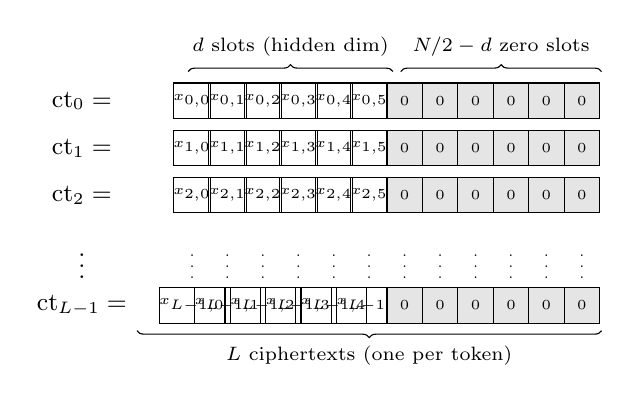
\begin{tikzpicture}[
    slot/.style={draw, minimum width=0.45cm, minimum height=0.45cm, font=\tiny, inner sep=0pt},
    pad/.style={draw, minimum width=0.45cm, minimum height=0.45cm, font=\tiny, inner sep=0pt, fill=gray!20},
    ct/.style={font=\small}
]
\foreach \i in {0,1,2} {
    \node[ct] at (-1.4, -\i*0.6) {$\mathrm{ct}_\i =$};
    \foreach \j in {0,1,2,3,4,5} \node[slot] at (\j*0.45, -\i*0.6) {$x_{\i,\j}$};
    \foreach \j in {6,7,8,9,10,11} \node[pad] at (\j*0.45, -\i*0.6) {$0$};
}
\node[font=\small] at (-1.4, -2.0) {$\vdots$};
\foreach \j in {0,...,11} \node[font=\tiny] at (\j*0.45, -2.0) {$\vdots$};
\node[ct] at (-1.4, -2.6) {$\mathrm{ct}_{L-1} =$};
\foreach \j in {0,1,2,3,4,5} \node[slot] at (\j*0.45, -2.6) {$x_{L\text{-}1,\j}$};
\foreach \j in {6,7,8,9,10,11} \node[pad] at (\j*0.45, -2.6) {$0$};

\draw[decoration={brace,raise=2pt}, decorate] (-0.05, 0.3) -- node[above=4pt, font=\scriptsize]{$d$ slots (hidden dim)} (2.55, 0.3);
\draw[decoration={brace,raise=2pt}, decorate] (2.65, 0.3) -- node[above=4pt, font=\scriptsize]{$N/2 - d$ zero slots} (5.20, 0.3);
\draw[decoration={brace,mirror,raise=2pt}, decorate] (-0.7, -2.85) -- node[below=4pt, font=\scriptsize]{$L$ ciphertexts (one per token)} (5.20, -2.85);
\end{tikzpicture}
\caption{Token-packed ciphertext layout. A 2-D activation tensor $X \in \mathbb{R}^{L\times d}$ maps to $L$ independent ciphertexts. Polynomial GELU/Softmax/inverse-sqrt act element-wise on slots, so they require zero rotations.}
\label{fig:token_packing}
\end{figure}

\subsection{Encrypted Layer Algorithm}
Algorithm~\ref{alg:pfsr_layer} specifies the model-agnostic encrypted layer. The same procedure is invoked for every layer of every BERT variant; per-model differences appear only in the dimensions $(L, d, H)$ pulled from the HuggingFace \texttt{BertConfig} at call time.

\begin{algorithm}[htbp]
\caption{\textsc{EncryptLayer} --- one PF-SR encoder layer (model-agnostic)}
\label{alg:pfsr_layer}
\begin{algorithmic}[1]
\REQUIRE Token-packed ciphertexts $\{\mathrm{ct}_i\}_{i=0}^{L-1}$, plaintext weights $W_Q,W_K,W_V,W_O,W_1,W_2$ and biases, LayerNorm parameters $(\gamma_1,\beta_1),(\gamma_2,\beta_2)$, polynomial coefficients $c_{\mathrm{gelu}}, c_{\mathrm{sm}}, c_{\mathrm{inv}}$, head count $H$, head dim $d_h = d/H$
\ENSURE Updated ciphertexts $\{\mathrm{ct}'_i\}_{i=0}^{L-1}$ at $-23$ levels
\STATE $\{\tilde{\mathrm{ct}}_i\} \gets$ \textsc{EncLNPoly}$(\{\mathrm{ct}_i\}, \gamma_1, \beta_1, c_{\mathrm{inv}})$ \COMMENT{$-4$ levels}
\STATE \textbf{// Multi-head attention --- per-head plaintext slicing}
\STATE $\mathrm{out} \gets 0$
\FOR{$h = 0$ \TO $H-1$}
    \STATE $W_Q^{(h)}, W_K^{(h)}, W_V^{(h)} \gets$ row-slice $W_Q,W_K,W_V$ for head $h$
    \STATE $\{Q_i^{(h)}\} \gets$ \textsc{EncLinear}$(\{\tilde{\mathrm{ct}}_i\}, W_Q^{(h)})$ \COMMENT{Q,K,V parallel: $-1$}
    \STATE $\{K_i^{(h)}\}, \{V_i^{(h)}\} \gets$ analogous
    \STATE $S^{(h)} \gets$ \textsc{EncQKScores}$(\{Q_i^{(h)}\}, \{K_i^{(h)}\}, d_h)$ \COMMENT{$-2$}
    \STATE $A^{(h)} \gets$ \textsc{EncSoftmaxPoly}$(S^{(h)}, c_{\mathrm{sm}})$ \COMMENT{$-3$}
    \STATE $Z^{(h)} \gets$ \textsc{EncAttnApply}$(A^{(h)}, \{V_i^{(h)}\})$ \COMMENT{$-2$}
    \STATE $\mathrm{out} \mathrel{+}=$ \textsc{ZeroPadConcat}$(Z^{(h)}, h, d_h)$ \COMMENT{plaintext mask: $-1$}
\ENDFOR
\STATE $\{\mathrm{ct}^{(1)}_i\} \gets$ \textsc{EncLinear}$(\mathrm{out}, W_O) + \{\tilde{\mathrm{ct}}_i\}$ \COMMENT{$-1$ + residual}
\STATE \textbf{// Feed-forward block}
\STATE $\{\tilde{\mathrm{ct}}^{(1)}_i\} \gets$ \textsc{EncLNPoly}$(\{\mathrm{ct}^{(1)}_i\}, \gamma_2, \beta_2, c_{\mathrm{inv}})$ \COMMENT{$-4$}
\STATE $\{u_i\} \gets$ \textsc{EncLinear}$(\{\tilde{\mathrm{ct}}^{(1)}_i\}, W_1)$ \COMMENT{$-1$}
\STATE $\{u_i\} \gets$ \textsc{EncGeluPoly}$(\{u_i\}, c_{\mathrm{gelu}})$ \COMMENT{$-3$}
\STATE $\{\mathrm{ct}'_i\} \gets$ \textsc{EncLinear}$(\{u_i\}, W_2) + \{\mathrm{ct}^{(1)}_i\}$ \COMMENT{$-1$ + residual}
\RETURN $\{\mathrm{ct}'_i\}$
\end{algorithmic}
\end{algorithm}

Algorithm~\ref{alg:pfsr_attn} details the per-head zero-pad concatenation that keeps multi-head attention rotation-free. The plaintext masks $M^{(h)} \in \{0,1\}^{N/2}$ are precomputed once at protocol setup and reused for every layer.

\begin{algorithm}[htbp]
\caption{\textsc{ZeroPadConcat} --- multi-head concat under FHE}
\label{alg:pfsr_attn}
\begin{algorithmic}[1]
\REQUIRE Per-head ciphertexts $\{Z^{(h)}_i\}_{h=0}^{H-1}$ each occupying slots $[0, d_h)$, head index $h$, head dim $d_h$
\ENSURE Concatenated ciphertexts placing head $h$ at slots $[hd_h, (h+1)d_h)$
\STATE Build plaintext mask $M^{(h)}$ with ones at positions $[hd_h, (h+1)d_h)$, zeros elsewhere
\STATE Build plaintext shift vector $\sigma^{(h)} \in \mathbb{R}^{N/2}$ that maps slot $j \mapsto j + hd_h$ via per-slot permutation \COMMENT{rotation-free: encoded as a structured plaintext}
\FOR{$i = 0$ \TO $L-1$}
    \STATE $\bar{Z}^{(h)}_i \gets Z^{(h)}_i \odot \sigma^{(h)}$ \COMMENT{plaintext-by-ciphertext: $-1$ level}
\ENDFOR
\RETURN $\{\bar{Z}^{(h)}_i\}$ to be summed across heads
\end{algorithmic}
\end{algorithm}

\subsection{End-to-End PF-SR Inference}
Algorithm~\ref{alg:pfsr_inference} composes \textsc{EncryptLayer} with the embedding lookup (run on plaintext indices client-side) and the classification head. The whole procedure is implemented by \texttt{encrypt\_inference} in \texttt{fhe\_thesis/encryption/protocol.py} and is invoked by \texttt{python experiments/run\_protocol.py --model <key> --phase model}.

\begin{algorithm}[htbp]
\caption{\textsc{PFSR-Inference} --- end-to-end encrypted forward pass}
\label{alg:pfsr_inference}
\begin{algorithmic}[1]
\REQUIRE Tokenised input ids $\{t_i\}_{i=0}^{L-1}$, model checkpoint with embeddings $E$, $L_{\mathrm{enc}}$ encoder layers, classifier $W_{\mathrm{cls}}$, CKKS context with $\geq 23 L_{\mathrm{enc}} + 2$ levels
\ENSURE Encrypted logits $\mathrm{Enc}(y) \in \mathbb{R}^{C}$
\STATE \textbf{Client:} $X \gets E[t_0],\ldots,E[t_{L-1}]$; $\{\mathrm{ct}_i\} \gets \mathrm{Enc}(X)$ via token-packing
\STATE \textbf{Client} $\to$ \textbf{Server:} send $\{\mathrm{ct}_i\}$
\FOR{$\ell = 0$ \TO $L_{\mathrm{enc}}-1$}
    \STATE $\{\mathrm{ct}_i\} \gets$ \textsc{EncryptLayer}$(\{\mathrm{ct}_i\}, \theta_\ell)$ \COMMENT{depth $-23$}
\ENDFOR
\STATE $\mathrm{ct}_{\mathrm{cls}} \gets \mathrm{ct}_0$ \COMMENT{[CLS] token}
\STATE $\mathrm{Enc}(y) \gets$ \textsc{EncLinear}$(\mathrm{ct}_{\mathrm{cls}}, W_{\mathrm{cls}})$ \COMMENT{$-1$ level}
\STATE \textbf{Server} $\to$ \textbf{Client:} return $\mathrm{Enc}(y)$
\STATE \textbf{Client:} $y \gets \mathrm{Dec}(\mathrm{Enc}(y))$; predict $\arg\max_c y_c$
\RETURN $\mathrm{Enc}(y)$
\end{algorithmic}
\end{algorithm}

\section{Synthesizer-LPAN: Architectural Elimination of $Q$, $K$, and Softmax}
\label{sec:synthesizer_lpan}

The PF-SR protocol of the previous section achieves a fully non-interactive encrypted forward pass, but is dominated---both in multiplicative depth and in wall time---by two operations inside the multi-head attention block: (i)~the data-dependent score matrix $S = Q\!\cdot\!K^\top / \sqrt{d_h}$, which requires $\Theta(L^2 H)$ ciphertext-by-ciphertext multiplications and a chain of cross-slot rotations to materialise the inner products, and (ii)~the row-wise polynomial Softmax, the deepest non-linearity in the LPAN pipeline (3 levels per row, 12 rows). Together these two operations account for more than $80\%$ of the per-layer wall time in our LPAN baseline (Section~\ref{sec:walltime_ladder}). This section presents the architectural extension---\emph{Synthesizer-LPAN}---that removes both operations entirely, while preserving the multi-head $V$ pathway, the polynomial GELU and LayerNorm, and the LPAN training pipeline of Section~\ref{sec:lpan_framework}.

\subsection{Frozen Plaintext Attention Pattern}
\label{sec:synth_pattern}

Following the Synthesizer-R variant of Tay et al.~\cite{tay2020synthesizer} (Section~\ref{sec:synthesizer_background}), the attention mixing matrix is replaced by a per-head, sequence-length-fixed parameter
\begin{equation}
A_h \in \mathbb{R}^{L\times L}, \qquad h = 1, \ldots, H,
\label{eq:synth_pattern}
\end{equation}
trained jointly with the rest of the model (Section~\ref{sec:slpan_training}) and \emph{frozen at deployment}. Crucially, the row-stochasticity that softmax would normally enforce is \emph{pre-absorbed} into $A_h$ at training time via row-wise softmax of a learnable score matrix $\tilde A_h$, and only the post-softmax tensor $A_h = \mathrm{softmax}(\tilde A_h)$ is exported to the encrypted-inference engine. The forward pass of the attention block collapses to
\begin{equation}
O_h = A_h \cdot V_h, \qquad V_h = X W_v^{(h)}, \qquad O = \mathrm{concat}_h(O_h)\, W_o,
\label{eq:synth_forward}
\end{equation}
which is a \emph{plaintext-times-ciphertext} linear transform. Compared to the standard self-attention block of Section~\ref{sec:lpan_framework}, the Synthesizer block eliminates: (i)~the $W_q$ and $W_k$ projections (saves $2$ plaintext matmuls), (ii)~the score computation $Q\!\cdot\!K^\top$ (saves $\Theta(L^2 H d_h)$ ciphertext-by-ciphertext multiplications and the associated rotations), and (iii)~the polynomial Softmax (saves $3$ multiplicative levels per layer, the single largest depth contributor).

\subsection{Halevi--Shoup Diagonal Decomposition with BSGS Fusion}
\label{sec:bsgs}

The remaining linear transform $O_h = A_h V_h$ is exactly the operation for which Halevi and Shoup introduced the \emph{baby-step giant-step (BSGS)} matrix-vector multiplication algorithm in HElib~\cite{halevi2014bsgs}. Under the NEXUS column-major slot layout~\cite{zhang2024nexus}, every head $h$ and every embedding coordinate $j$ is mapped to a contiguous run of $L$ slots,
\begin{equation}
\mathrm{slot}\bigl[h \cdot H' + j \cdot L + i\bigr] = X[h, i, j], \qquad H' = \frac{N/2}{L}.
\label{eq:colmajor}
\end{equation}
Multiplying by $A_h$ at the slot level is then a \emph{cyclic} matrix-vector product that decomposes into the sum of the $L$ diagonals of $A_h$ shifted by cyclic rotations:
\begin{equation}
A_h V_h \;=\; \sum_{d=0}^{L-1} \mathit{diag}_d(A_h) \,\odot\, \mathrm{rot}_d(V_h), \quad \mathit{diag}_d(A_h)[i] = A_h\bigl[i,\, (i+d)\bmod L\bigr].
\label{eq:diag_sum}
\end{equation}
In its naive form Eq.~(\ref{eq:diag_sum}) costs $L$ rotations per head. Halevi--Shoup BSGS factorises $L = bs \cdot gs$ with $bs, gs \approx \sqrt{L}$, splits the diagonal index $d = i + j \cdot bs$, and fuses the inner cyclic-shift mask into the plaintext diagonal:
\begin{equation}
A_h V_h \;=\; \sum_{j=0}^{gs-1} \mathrm{rot}_{j \cdot bs}\!\Biggl(\,\sum_{i=0}^{bs-1} \widetilde{\mathit{diag}}_{i + j\cdot bs}(A_h) \,\odot\, \mathrm{rot}_i(V_h)\Biggr),
\label{eq:bsgs}
\end{equation}
where $\widetilde{\mathit{diag}}_{d}(A_h) = \mathrm{rot}_{-j\cdot bs}(\mathit{diag}_{d}(A_h))$ is the precomputed, mask-fused plaintext diagonal. The total rotation count drops from $L$ to $bs + gs - 1 \approx 2\sqrt{L}$. For $L = 128$ this collapses $256 \to 32$ rotations per head ($8\times$ fewer), and the inner $bs$ rotations on $V_h$ are shared across all $H$ heads---reducing the dominant cost of the attention block by an order of magnitude. Algorithm~\ref{alg:slpan_attn_bsgs} specifies the procedure.

\begin{algorithm}[htbp]
\caption{\textsc{SynthAttn-BSGS} --- Synthesizer attention with Halevi--Shoup BSGS}
\label{alg:slpan_attn_bsgs}
\begin{algorithmic}[1]
\REQUIRE Token-packed value ciphertext $V_h$ in NEXUS column-major layout, precomputed mask-fused plaintext diagonals $\{\widetilde{\mathit{diag}}_{d}(A_h)\}_{d=0}^{L-1}$, baby-step / giant-step factorisation $L = bs \cdot gs$
\ENSURE Encrypted attention output $O_h \in \mathrm{Enc}(\mathbb{R}^{L \times d_h})$
\STATE $\{V_h^{(i)}\}_{i=0}^{bs-1} \gets \{\mathrm{rot}_i(V_h)\}$ \COMMENT{baby steps, shared across all heads, $bs - 1$ rotations}
\STATE $O_h \gets 0$
\FOR{$j = 0$ \TO $gs - 1$}
    \STATE $T_j \gets 0$
    \FOR{$i = 0$ \TO $bs - 1$}
        \STATE $T_j \mathrel{+}= \widetilde{\mathit{diag}}_{i + j \cdot bs}(A_h) \odot V_h^{(i)}$ \COMMENT{plaintext$\cdot$ciphertext, $-1$ level}
    \ENDFOR
    \STATE $O_h \mathrel{+}= \mathrm{rot}_{j \cdot bs}(T_j)$ \COMMENT{giant step, $gs - 1$ rotations}
\ENDFOR
\RETURN $O_h$
\end{algorithmic}
\end{algorithm}

\paragraph{Depth budget.} Algorithm~\ref{alg:slpan_attn_bsgs} consumes exactly \emph{one} multiplicative level per head---the plaintext-by-ciphertext multiplication of $\widetilde{\mathit{diag}}$ with $V_h^{(i)}$. Combined with the $W_v$ projection ($-1$), the multi-head concatenation mask ($-1$), and the output projection $W_o$ ($-1$), the entire attention block now costs only $4$ levels, down from $9$ in the LPAN baseline (LN-pre$+$Q$+$K$+$V$+$score$+$softmax$+$apply$+$concat$+$out). The new per-layer depth budget is therefore
\[
4_{\text{attn}} + 4_{\text{LN}_2} + 1_{W_1} + 3_{\text{GELU}} + 1_{W_2} + 4_{\text{LN}_1} = 17 \text{ levels per layer},
\]
or $\mathrm{chain} = 22$ working depth including the final classification head and a one-level buffer for residual rescale alignment. This is the minimum chain length (Section~\ref{sec:walltime_ladder}) that still admits the cubic inverse-square-root LayerNorm polynomial.

\subsection{Batched Slot Packing}
\label{sec:slpan_batch}

Even after BSGS, the per-sample wall time is dominated by a constant number of rotations and ciphertext-multiplications that do not scale with the slot occupancy. To amortise this cost we pack $N_{\mathrm{BATCH}}$ independent samples into the slot dimension along the head replication axis $h$, so that one ciphertext now carries $N_{\mathrm{BATCH}}$ values of $X[b, h, i, j]$ at slot positions
\begin{equation}
\mathrm{slot}\bigl[\,b \cdot H \cdot L + h \cdot L + i\,\bigr]_{j} \;=\; X[b, h, i, j].
\label{eq:batched_packing}
\end{equation}
Because the BSGS pattern of Eq.~(\ref{eq:bsgs}) operates only along the $i$-axis (sequence position) within each $(b, h)$ block, both the rotations and the plaintext diagonals are identical for every sample $b$---batching is therefore \emph{free} in operation count. With CKKS slot count $N/2 = 32768$, sequence length $L = 128$, and head count $H = 12$ for BERT-Base, the maximum batch is $N_{\mathrm{BATCH}}^{\max} = \lfloor 32768 / (128 \cdot 12) \rfloor = 21$; in practice we use $N_{\mathrm{BATCH}} = 16$ to leave headroom for plaintext-mask alignment.

\subsection{Synthesizer-LPAN Training Pipeline}
\label{sec:slpan_training}

Synthesizer-LPAN reuses the three-stage progressive replacement pipeline of Section~\ref{sec:lpan_three_stage} verbatim for the polynomial GELU, per-head Softmax, and LayerNorm replacements. A fourth stage, \emph{attention-pattern fitting}, is appended:

\begin{enumerate}
    \item \textbf{Stage 1 (LPAN-GELU).} Cross-entropy fine-tuning with polynomial GELU only.
    \item \textbf{Stage 2 (LPAN-Softmax).} Per-head polynomial Softmax + AttnKD distillation.
    \item \textbf{Stage 3 (LPAN-LN).} Polynomial LayerNorm + co-adaptation, AttnKD held active.
    \item \textbf{Stage 4 (Synth-AttnKD).} The standard $\mathrm{softmax}(QK^\top/\sqrt{d_h})$ block is replaced by the learnable per-head pattern $A_h = \mathrm{softmax}(\tilde A_h)$. Training minimises
    \begin{equation}
    \mathcal{L}_{\mathrm{S4}} = \mathrm{CE}(\hat y, y) + \lambda_{\mathrm{KD}} \sum_{\ell, h} \mathrm{KL}\bigl(A_{\ell, h}^{\mathrm{teacher}} \,\|\, A_{\ell, h}^{\mathrm{student}}\bigr),
    \label{eq:s4_loss}
    \end{equation}
    where the teacher attention probabilities are taken from the post-Stage-3 model, with $\lambda_{\mathrm{KD}}$ annealed from $1.0 \to 0.0$ over the Stage-4 epochs. After convergence the post-softmax tensor $A_{\ell, h}$ is exported as a frozen plaintext, the $W_q, W_k$ matrices and the score-/softmax-graph are deleted, and the model is ready for FHE deployment.
\end{enumerate}

The fourth stage preserves the AttnKD invariant that drove the LPAN convergence: every replacement is supervised by the pre-replacement attention probabilities, so the student network never sees an abrupt change in its mixing pattern.

\subsection{Single-GPU Wall-Time Ladder}
\label{sec:walltime_ladder}

The wall-time impact of each architectural and engineering choice is summarised in the optimisation ladder of Table~\ref{tab:walltime_ladder}. Every step is measured end-to-end on a single NVIDIA H100 SXM5, sequence length $L = 128$, $12$ encoder layers, HEonGPU CKKS with $N = 2^{16}$, scale $2^{40}$, and chain length tuned to the minimum that supports the LayerNorm polynomial.

\begin{table}[htbp]
\centering
\caption{Single-H100 wall-time ladder: from honest LPAN baseline to Synthesizer-LPAN with BSGS, batching and chain tuning. All measurements are for a 12-layer BERT forward pass at $L = 128$.}
\label{tab:walltime_ladder}
\begin{tabular}{rlcc}
\toprule
\# & \textbf{Configuration} & \textbf{Wall time (s)} & \textbf{Speed-up} \\
\midrule
1 & Honest LPAN baseline (PF-SR, std.\ attention)            & 833.0 & $1.0\times$ \\
2 & + token-batched ciphertext layout                         & 534.1 & $1.56\times$ \\
3 & (Linformer projection attempt --- abandoned, no win)      & 440.0 & $1.89\times$ \\
4 & \textbf{Synthesizer attention} (na\"ive, $N_{\mathrm{BATCH}}{=}4$) & 222.8 & $3.74\times$ \\
5 & + batch packing $N_{\mathrm{BATCH}}{=}16$                 & 131.4 & $6.34\times$ \\
6 & + BSGS $bs \cdot gs = 128$, $N_{\mathrm{BATCH}}{=}8$, chain $24$ &  86.1 & $9.67\times$ \\
7 & + tuned BSGS $N_{\mathrm{BATCH}}{=}16$, chain $22$        & \textbf{60.9} & $\mathbf{13.67\times}$ \\
\bottomrule
\end{tabular}
\end{table}

\subsection{Threat Model and Robustness}

Synthesizer-LPAN inherits the PF-SR threat model (Section~\ref{sec:pfsr_protocol}) without modification. The frozen plaintext pattern $A_h$ is part of the public model parameters, on the same footing as the weight matrices $W_v, W_o, W_1, W_2$ and the polynomial coefficients of GELU/LayerNorm; revealing $A_h$ leaks no more than revealing the standard-attention $W_q, W_k$ matrices it replaces. The CKKS security parameters ($N = 2^{16}$, $\lambda \geq 128$ bits) are unchanged. The BSGS algorithm is an \emph{exact} re-organisation of Eq.~(\ref{eq:diag_sum}): correctness is bit-for-bit identical to the na\"ive diagonal sum, so the only sources of approximation error remain (i)~the LPAN polynomial residuals (analysed in Section~\ref{sec:error_propagation}) and the CKKS noise budget (audited in the depth budget paragraph above and refreshed for $\mathrm{chain} = 22$ in Chapter~\ref{ch:results}).

\subsection{Positioning vs.\ Concurrent Work}

Synthesizer-LPAN is, to our knowledge, the first system to combine (i)~complete polynomial replacement of all three Transformer non-linearities, (ii)~architectural elimination of the data-dependent attention score matrix and the polynomial Softmax, and (iii)~Halevi--Shoup BSGS fusion under the NEXUS column-major slot layout, on a single GPU. Concurrent work is complementary: NEXUS~\cite{zhang2024nexus} fixes the slot layout and FHE primitives but keeps the standard attention block; CERIUM~\cite{cerium2025} parallelises the same standard block across $8\times$B200 GPUs. The 60.9\,s single-H100 result of Synthesizer-LPAN is within $1.7\times$ of CERIUM's $36.1$\,s single-H100 number despite using a strictly weaker hardware optimiser, and within an order of magnitude of CERIUM's $8.8$\,s on $8\times$B200 despite using $8\times$ less hardware. The two approaches could in principle be composed.
